\section{Introduction}
The work presented in this thesis, being experimental in nature, hinges on numerous experimental techniques. The fundamental components of this work rely upon extensive use of X-ray diffraction (XRD) and transmission electron microscopy (TEM) in non-standard and novel ways. These techniques will be examined and examined in some detail, as their novel usage is integral to the work presented here. Several other experimental techniques are also utilized in this work, but they are used in their everyday implementations as seen in many papers in literature. These experimental techniques will be discussed only briefly for brevity. The two primary growth techniques used in this work will also be described, however as this work concentrates on epitaxy is a general phenomenon the intricacies and parameter spaces of these techniques will not be considered again for brevity.

\section{X-Ray}
X-rays are high energy photons, generated from the transitions of electrons between their core shell energy levels and bremsstrahlung (the acceleration of electrons). X-rays have a relatively weak interaction with matter, being absorbed or perturbed only slightly upon passing through it. X-rays have wavelengths comparable with the typical spacings between atoms in crystals, placing them as an ideal non-destructive probe for crystal structure. X-rays experience elastic scattering when interacting with the electrons surrounding atoms. The scattering of x-rays, combined with the 3D periodic structure of atoms, results in constructive and destructive interference and x-ray diffraction.
\begin{equation}
\label{eqn:bragg} 2d \sin(\theta) = n \lambda
\end{equation}
X-ray diffraction is fundamentally an interference phenomenon, for a set of planes within a crystal separated by some distance (d), they will diffract from those planes at an angle (\texttheta) depending upon the wavelength (\textlambda), this is known as Bragg's law as in \cref{eqn:bragg}. Bragg's law is identical to the phenomenon of thin film interference of visible light, only differing by the scale of the spacing and wavelengths. Bragg's law, while correct, is a one dimensional expression, in general it can be represented by the Laue Equations as in \cref{eqn:laue}. The vectors $k_i$ and $k_0$ are the incident and outgoing x-ray beam, $(a,b,c)$ is the primitive vector of the crystal lattice and $(h,k,l)$ are the reciprocal lattice indicies which must be integers. Thus, for a given crystal with a fixed unit cell, there are only certain relationships between the incident and outgoing x-ray beams that satisfy the diffraction conditions, resulting in diffraction.
\begin{align}
   a \cdot (k_0 - k_i) = 2 \pi h \\
   b \cdot (k_0 - k_i) = 2 \pi k \\
   c \cdot (k_0 - k_i) = 2 \pi l
   \label{eqn:laue}
\end{align}

A concept known as reciprocal, or momentum space, is a common construct used in solid state physics to discuss the properties of crystals and is intimately related to diffraction. Reciprocal space can be visualized as a lattice of points, each representing a spacing present in the crystal, and the lattice having the same symmetry as the real crystal. Reciprocal space is also the Fourier partner of the real space lattice of the crystal. Reciprocal space provides an opportunity for an alternate expression of the conditions for diffraction, known as the Ewald construction. The Ewald construction or Ewald sphere expresses the diffraction condition through the overlay of a sphere of radius 1/\textlambda{} pinned on its radius at the origin in reciprocal space, a incident X-ray beam ($k_i$) entering the sphere. The direction of the exiting diffraction beam is determined by the intersection of the surface of the sphere with the reciprocal lattice, as shown in \cref{fig:exp_xray_ewald}. As a crystal is rotated (or the incoming beam is moved), the Ewald sphere will rotate about the origin, sweeping through reciprocal space and exciting diffraction conditions as the sphere coincides with lattice points. The pinned rotation of the Ewald sphere about the origin means that only reciprocal lattice points with a radius from the origin of less than 2/\textlambda{} can be excited into diffraction, indicating the effective limitation of a given x-ray source, as well as why light is an ineffective diffraction probe.
\begin{figure}
\centering
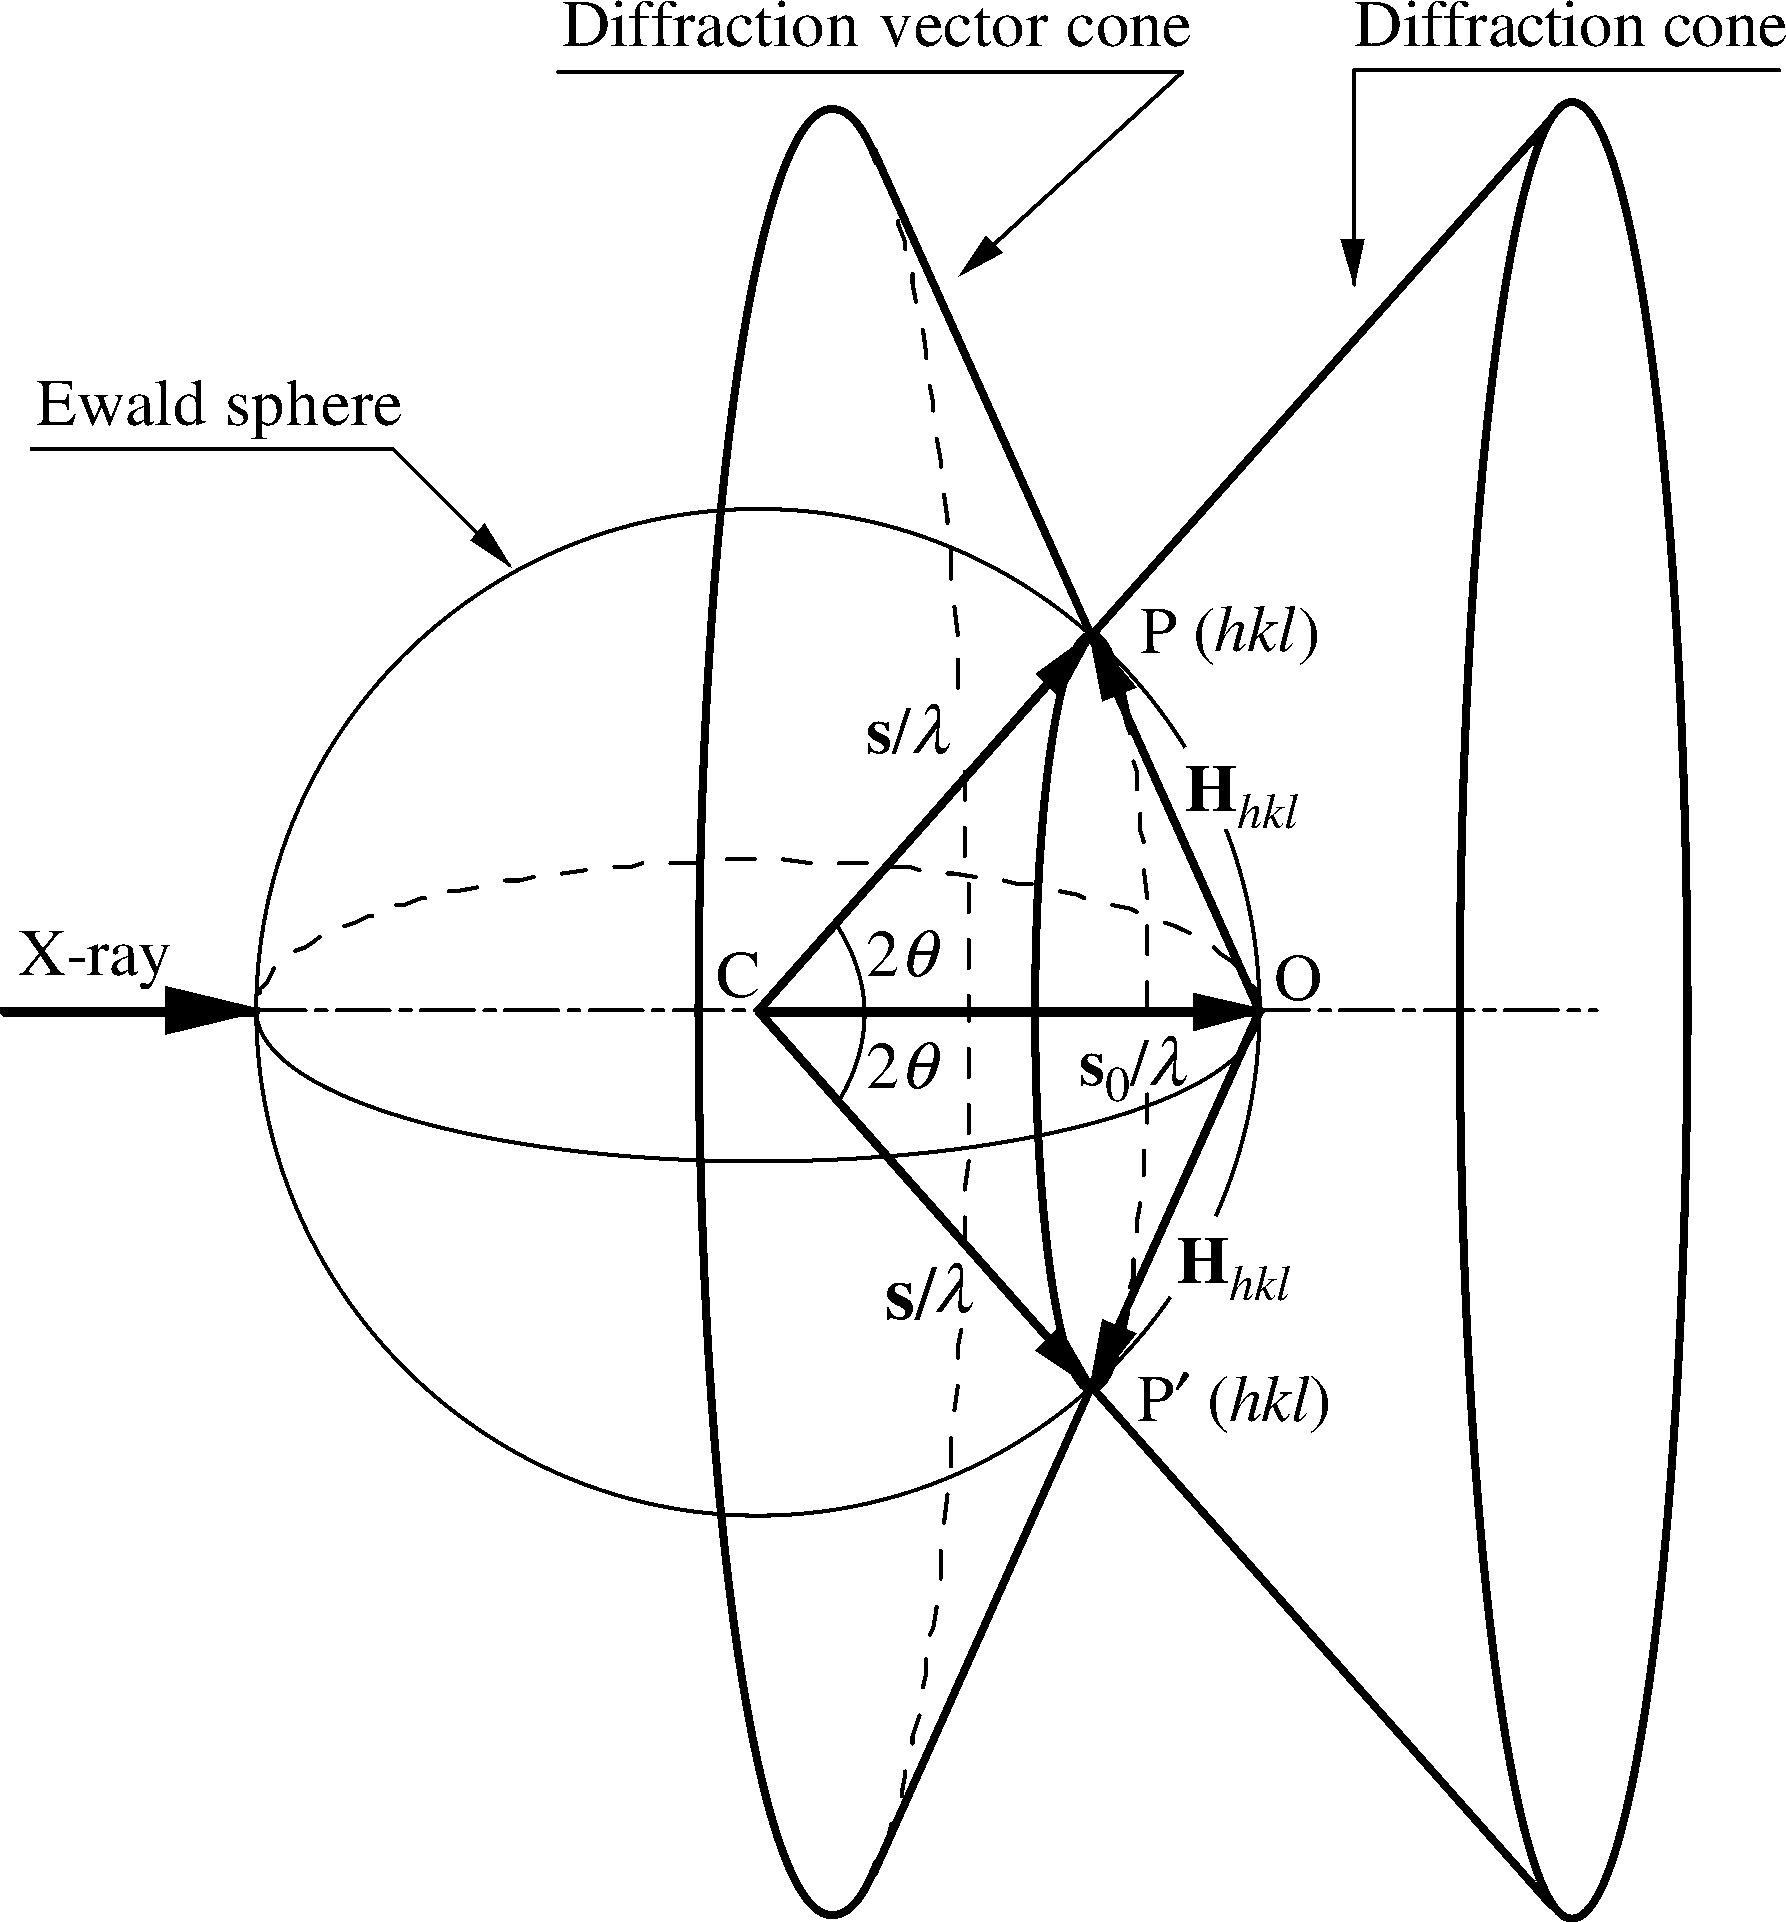
\includegraphics[width=0.8\textwidth]{exp_xray_ewald}
\caption{\label{fig:exp_xray_ewald}Ewald sphere construction of diffraction conditions\cite{bobhe}}
\end{figure}

\subsection{2DXRD - Reciprocal Space Mapping}
\label{sec:2DXRD} As shown by \cref{eqn:laue} and \cref{fig:exp_xray_ewald}, there are an large number of orientations of a crystal which generate diffraction. For the purposes of the analysis of crystals, the lowest orders of crystal diffraction (small h,k,l) are the strongest, and provide the least ambiguous information, the they are also at the lowest 2\texttheta{} values. This still leaves a significant number of diffraction beams of interest to measure and provide structural information. The naive measurement technique for collecting this information involves taking a crystal and orienting an incoming x-ray beam, and a detector in configurations that satisfy \cref{eqn:laue}. Such measurements assume that the experimenter knows the orientation and unit cell of the crystal to a degree well enough calculate those configurations. If either of those pieces of information is unknown, the experimenter must instead sample the 4\textpi{} solid angle (usually only the upper 2\textpi{} half) of angular space surrounding a crystal with sufficient resolution to intersect with the diffraction conditions of interest. Such experiments, when performed using a typical x-ray point detector, take inordinate amounts of time, as the angular space is large and the point detector must count for a long time to achieve good counting statistics.

An alternate implementation of such a measurement process is through the use of a 2D planar detector rather than a point detector. A 2D x-ray detector can subtend a large section the angular space surrounding a given experiment, potentially collecting information about a large section of reciprocal space with each frame it collects. If configuration is then swept through a range of diffraction conditions, the 2D detector will collect information about a wide swath of reciprocal space. 2DXRD techniques simultaneously collect information about the phase and symmetry of an unknown sample allowing that information to be then examined via a variety of techniques.

\subsubsection{Practical 2DXRD Measurement}
\begin{figure}
    \centering
    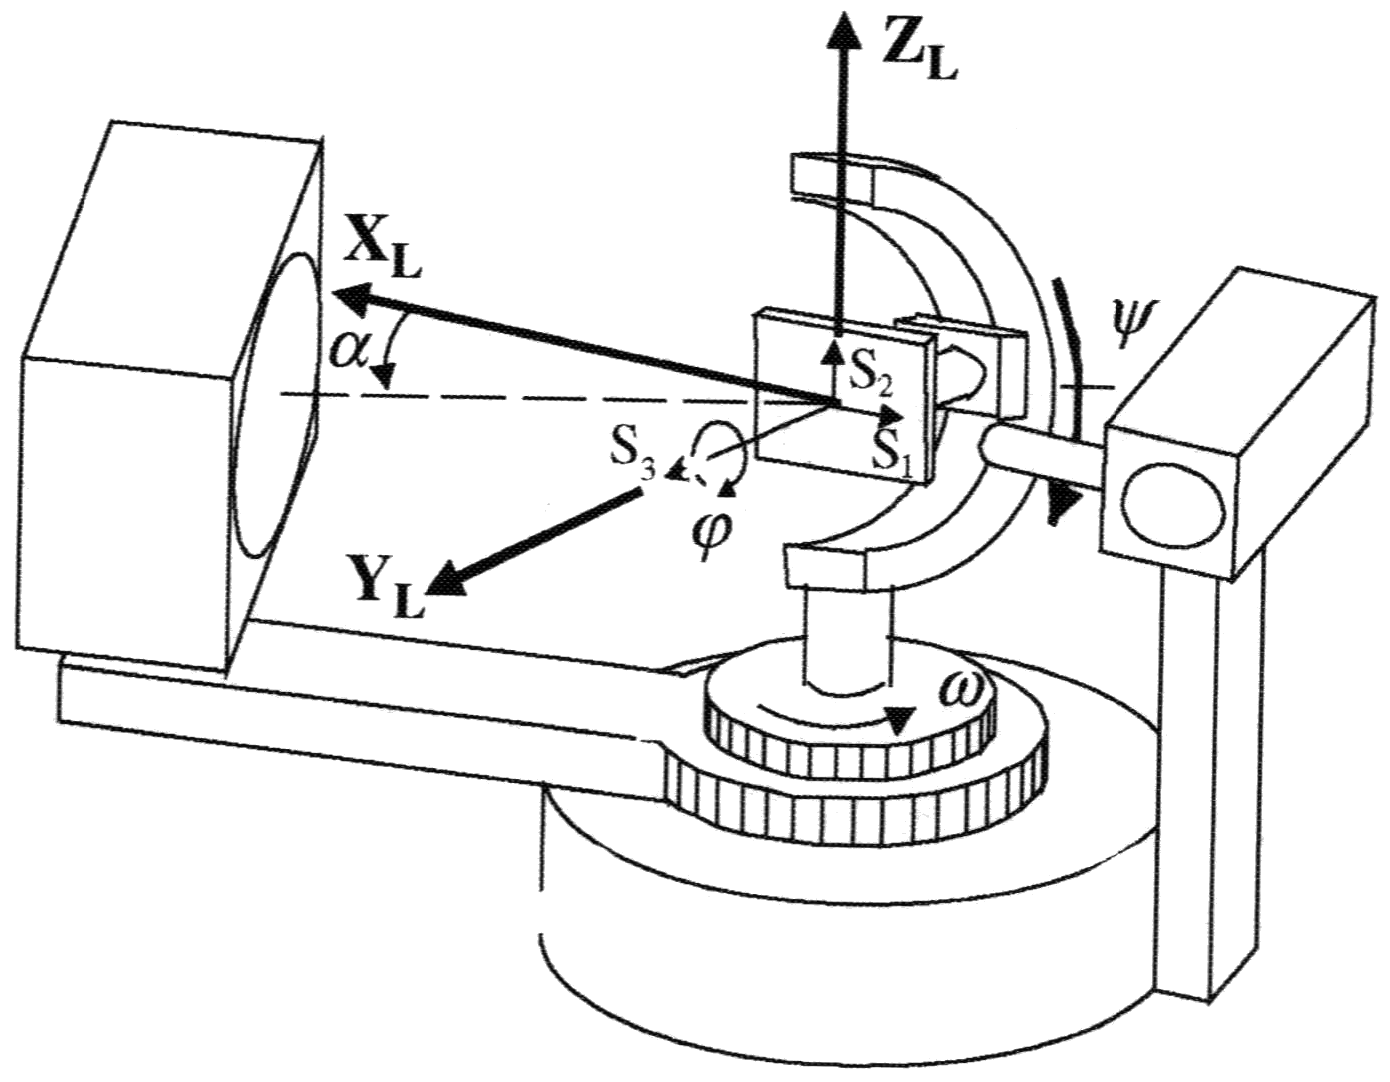
\includegraphics[width=0.8\textwidth]{exp_xray_machine}
    \caption{\label{fig:exp_xray_machine}Standard configuration of a 2DXRD system, with the laboratory geometry\cite{bobhe}}
\end{figure}
Practical 2DXRD measurements are achieved through the use of a multi-axis goiniometer, a device which maintains the sample at a central point while rotating its orientation relative to the X-ray source and detector. For the purposes of epitaxial crystals grown on substrates, a sample under measurement is placed in the goinometer with its surface normal oriented along the goiniometer's sample axis and a reference edge. An x-ray source is placed on one arm of the goiniometer and the 2D detector is placed on the other arm.

A standard 2DXRD measurement is performed by configuring the goiniometer (\cref{fig:exp_xray_machine}) such that the X-ray source to 2D detector angle corresponds to a known or presumed low-order 2\texttheta{} angle for the sample. The sample was then rotated such that incident angle relative to the surface is shallow, less than 5\degree{}. The sample would then be rotated about its surface normal while the 2D detector took sequential images, a process known as a \textphi{}-scan. By aligning the sample along 2\texttheta{} in one dimension, as the sample rotates in a complimentary dimension crystallographic directions that contain the d-spacing corresponding to a range of 2\texttheta{} around the selected value will be collected on the detector. An additional scan of the sample while maintaining the 2\texttheta{} configuration and scanning the X-ray beam incident angle is known as an \textomega{}-scan.

As the reciprocal space mapping is a process which operates in angular space, the distance the detector is an important optimization parameter for 2DXRD measurements. The distance the 2DXRD detector is situated away from sample will change the solid angle subtended by the detector. Close detector distances allow the collection of more reciprocal space data in a given scan, at the expense of reducing the resolution due to finite pixel size, as well as increasing the risk of overlap. For epitaxial thing films grown on lattice mismatched substrates, close detector distances can result in substrate and epitaxial crystal peaks overlapping, making interpretation difficult.
\subsubsection{Interpretation of 2DXRD Measurements}
\begin{figure}
    \centering
    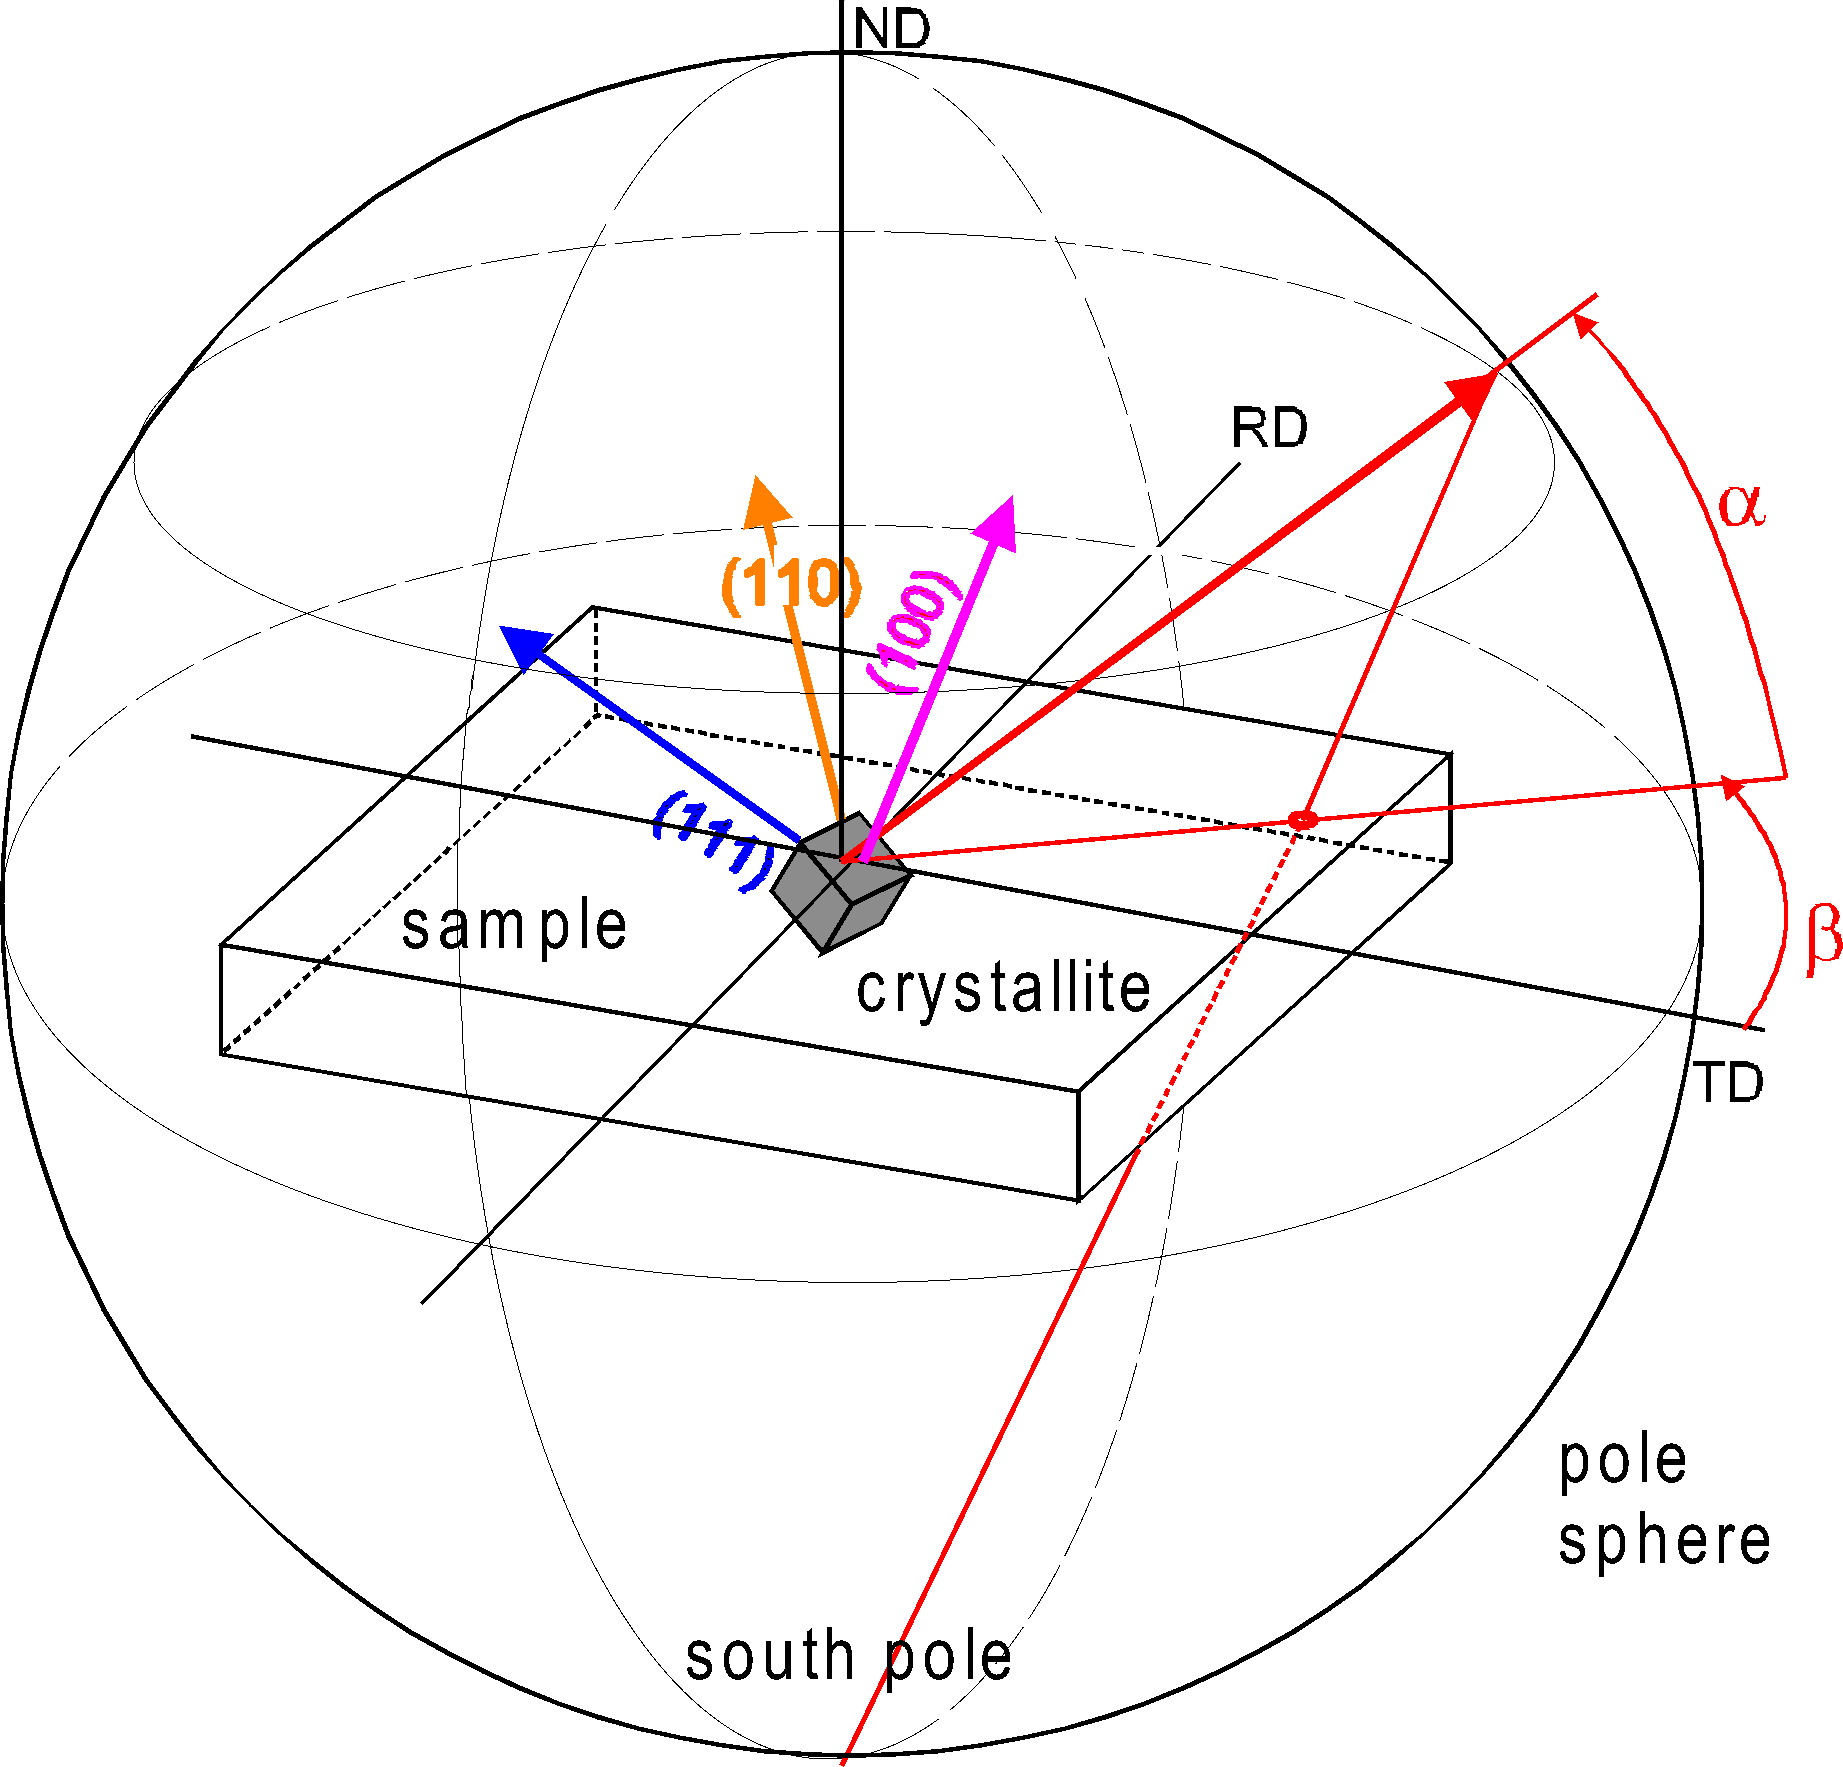
\includegraphics[width=0.9\textwidth]{exp_xray_polesphere}
    \caption{\label{fig:exp_xray_polesphere}The pole sphere showing the origin of peaks in a pole figure and their relationship to the sample and an individual unit cell\cite{gadds_manual}}
\end{figure}

\begin{figure}
    \centering
    \missingfigure{4 simulated pole figures, completely random, in-plane random, textured, single crystal}
    \caption{\label{fig:exp_xray_polefigure_examples}Example pole figures of a) Randomly oriented b) in-plane random orientation c) textured d) single crystal samples of the same composition and crystal structure}
\end{figure}


\subsection{High Resolution XRD}
While mapping reciprocal space provides a great deal of information about the phases and symmetries present in a given sample, the resolution available on such 2D detectors is limited in both the number of pixels, and the spacing between them. In addition, the x-ray beam geometry associated with 2DXRD measurements introduces instrumental broadening into the measurements preventing careful inspection of small scale diffraction details. In order to examine the small scale details of diffraction intensity, a different configuration must be implemented for the x-ray source and detector, this configuration is known as high resolution x-ray diffraction. If the general landscape of reciprocal space (diffraction intensity) is known through the application of 2DXRD techniques, HRXRD can carefully sample small sections of reciprocal space with very high resolution.

Recall that for a perfect crystal, there is only a single configuration for which the diffraction condition will be satisfied, resulting in a highly intense diffraction peak with minimal spacial extent. For a real sample, intensity distribution of individual diffraction peaks in reciprocal space provides information about the deviance from the ideal crystal.

Using HRXRD measurements, the exact d-spacing of a given material can be determined, showing whether a sample has its lowest energy structure or it is strained. If the orientation of the sample can be controlled carefully, the d-spacing can be measured absolutely, otherwise, it can be measured relative to a known standard such as a single crystal substrate. The broadening (spatial extent) of a HRXRD peak provides different information depending upon the dimension along which it is examined. In the 2\texttheta{} direction, the radial direction in reciprocal space, broadening indicates that the spacing of interest is actually a distribution of spacings within the region of the sample illuminated by x-rays. Such distributions can indicate strain or compositional variation in the region of interest. The broadness of the x-ray peak when sample is rocked in the \textomega{} direction, while keeping 2\texttheta{} fixed indicates that a given d-spacing has a distribution of orientations within the sample, usually indicating multiple crystallites.


\subsubsection{Practical HRXRD Measurement}
%Single wavelength
%Arcsecond resolution goiniometer
%Highly parallel source
%Typically surface parallel planes

\section{Electron Microscopy}
The second of two very useful probes for examining the properties of epitaxial thin films is electrons, specifically, electron beams generated for electron microscopy. The electron, unlike the x-ray is a particle which interacts fairly strongly with materials. Electrons can be generated and accelerated to high velocities, resulting in DeBroglie wavelengths orders of magnitude smaller than X-rays and as a a result can be confined or focused to sub-angstrom areas. The electron's use as a probe can be used as both a mechanism to produce excite other phenomena for study, or to measure the effect a given sample has on a beam of uniform electrons. For generic beam of nearly-monochromatic electrons, typical of electron microscopy, a number of interactions are possible for a sample of finite thickness, as shown in \cref{fig:exp_em_electron_interaction}. The interactions of electrons with a sample can provide both chemical and structural information with fine spatial resolution thanks to the tight control of electron beams.
\begin{figure}
    \centering
    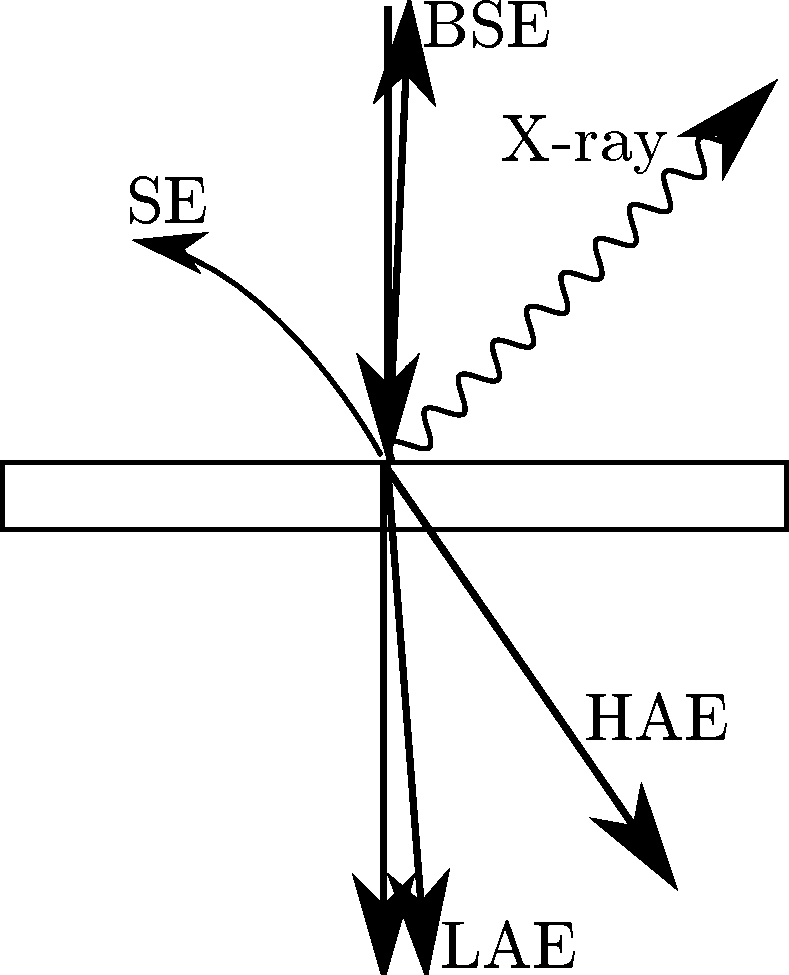
\includegraphics[width=0.7\textwidth]{exp_em_electron_interaction}
    \caption{\label{fig:exp_em_electron_interaction}Schematic of an electron beam interacting with a sample showing backscattered electrons (BSE), secondary electrons (SE), generated X-rays, low angle scattered electrons (LAE), high angle scattered electrons (HAE), and the main electron beam passing through the sample.}
\end{figure}

This work relied upon two measurement techniques which utilized electrons as their primary probe, scanning electron microscopy (SEM) and (scanning)transmission electron microscopy (STEM/TEM). SEM is an invaluable technique non-destructive technique for examining surfaces at high resolution to extract information about both the structural and chemical properties. STEM/TEM is a tool which utilizes similar interactions to examine the cross sectional structural and chemical properties of mechanically thinned slices of materials with sufficient resolution to examine individual columns of atoms in crystals.
\subsection{SEM}
Scanning electron microscopy is a high resolution non-destructive and non-contact technique used to examine the surface of a sample. SEM can provide information about the topography and chemical composition of a surface down to 10's of nanometers, and the exact chemical composition on the micrometer scale. These measurements are achieved through the interaction of a beam of nearly-monochromatic electrons generated from a heated filament or cold cathode and accelerated to kiloVolt velocities in an high vacuum chamber and focused onto a sample. Magnification is achieved in SEM by careful scanning of the focused beam over a small area.

\subsubsection{Secondary Electron Imaging}
The most common electron-material interaction utilized in SEM is generation of images through the production and capture of secondary electrons. Secondary electrons are continuum (valence and conduction band electrons) excited from the sample through inelastic scattering excitations. These electrons typically have energies of 10's to low 100's of electron volts. Secondary electrons are collected by biasing a electron detector in order to electrostatically attract these low energy electrons while not appreciably affecting the incoming beam. Electron detectors are typically a phosphor screen combined with a photomultipler tube to provide high gain. Images are formed by scanning the beam across the surface of the sample and counting the secondary electron yield for each dwell point within the scan. The resulting grid of counts is transformed into a grayscale image.

As secondary electrons are low energy, their escape depth from a surface is very shallow (< 2~nm), as such their yield is very sensitive to the local topography of the sample. Thus to the first approximation, the contrast in a grayscale image formed from secondary electrons is a representation of the topography present on the surface of the sample. Regions with vertical extent will increase the yield of secondary electrons, due to more of the sample being within nanometers of the surface. An extreme case of this is vertical edges, which will have a very high yield of secondary electrons, due to having the top and side surfaces both yielding secondary electrons.

\subsubsection{Backscattered Electron Imaging}
High energy incoming electrons can also interact with samples via elastic scattering. Electrons which are scattered at close to 90\degree{} are backscattered close to the incoming beam. By placing unbiased detector near the incoming electron beam the detector can capture backscattered electrons. The electron elastic scattering process is proportional to Z$^2$ of the sample. Thus the electron backscattering process forms an image that provides chemical contrast of the underlying sample.

\subsubsection{Practical SEM}
The practical application of SEM for imaging of samples requires the optimization of several parameters. While SEM is a non-destructive measurement technique, intentional sample preparation can vastly improve the imaging resolution and reduce noise. A key requirement for SEM samples is that the sample is suffciently conductive in order to conduct away the electrons delivered by the scanning beam. For high conductivity samples, sample preparation can be as simple as bonding to a sample holder using conductive tape or paste. Samples with poorer bulk conductivity may require conductive paste applied to contact the top surface to the sample holder. For highly insulating samples substrates are normally coated with a thin layer of high density metal (Pt, Au) or amorphous carbon in order to provide a conduction path.

Optimization of imaging for a given sample is achieved through the tuning of several imaging parameters, working distance, accelerating voltage, beam current and dwell time. For typical secondary electron imaging, the goal is to interact with the thin top surface layer with the smallest lateral beam possible. Minimization of accelerating voltage, beam current and working distance will maximize the resolution and reduce the surface interaction. Reduction of these working parameters has the side effect of reducing the signal to noise ratio (SNR) of imaging. Increasing dwell time can improve SNR, but for poorly conductive samples charge buildup will cause deflection of the incoming beam. Stacked averaging of quick scans yields improved SNR on the tradeoff of time. Interpretation of the secondary electron images in one key case is ambiguous, topographic features with vertical extent can be appear due to the human visual system to be both a depression and a bump alternately. Tilting of the sample can sometimes break the ambiguity and reveal the actual topography. Adjustment of the focus plane can also reveal the topography but only during active analysis.

Imaging of using backscattered electrons to achieve chemical composition requires optimization of the elastic scattering process from the sample. Backscattered electron yield increases with increasing accelerating voltage but also increases the area of interaction reducing resolution. The elastic scattering process is significantly less efficient than secondary electron generation, as such dwell times must be increased to yield an image. In order to obtain a true measure of chemical composition, samples for backscatter analysis should be as flat as possible, as topography can modify the yield of backscattered electrons. Such processing as polishing can improve the chemical contrast. If the measurement is intended to be non-destructive, careful correlation between backscattered and secondary electron images must be used to ignore topographic effects.
\subsection{TEM}

\subsection{STEM}


\section{Growth Techniques}
The work presented in this thesis are prepared primarily by two different growth methods, pulsed laser deposition (PLD) and molecular beam epitaxy (MBE). While these methods are quite distinct in their properties and the regimes under which they operate, the same material systems were not prepared by both systems, so direct comparisons cannot be made. Nevertheless, the differences between these growth processes will be examined in some detail to provide sufficient motivation for their choice for the given experiments.
\subsection{PLD}
\subsection{MBE}
\subsection{Thermal Dewetting}